\fancyhf{}
\fancyhead[LE,RO]{\small\textbf{\textsf{52}}}
\fancyhead[RE,LO]{\small\textsf{\textbf{CHƯƠNG 1}} \quad \textsf{Hàm số và Mô hình}}
\renewcommand{\headrulewidth}{0pt}

\noindent{\huge\textbf{\textsf{\color{stewartcyan}1.4}}}\quad {\Large\textbf{\textsf{Bài tập}}}
\vspace{0.8em}

\begin{multicols}{2}
\fontsize{8.2pt}{10.2pt}\selectfont
\setlength{\abovedisplayskip}{1.5pt}
\setlength{\belowdisplayskip}{1.5pt}



\noindent{\color{stewartcyan}\textbf{1--2}}\quad Sử dụng các Quy tắc Lũy thừa để viết lại và rút gọn từng biểu thức sau.

\vspace{0.3em}
\noindent\textbf{1.}
\begin{enumerate}[label=(\alph*),leftmargin=*,itemsep=2pt,topsep=1pt]
\item $\dfrac{-2^6}{4^3}$ \hfill (b) $\dfrac{(-3)^6}{9^6}$ \hfill (c) $\dfrac{1}{\sqrt[4]{x^5}}$
\item $\dfrac{x^3 \cdot x^n}{x^{n+1}}$ \hfill (e) $b^3(3b^{-1})^{-2}$ \hfill (f) $\dfrac{2x^2 y}{(3x^{-2} y)^2}$
\end{enumerate}

\vspace{0.3em}
\noindent\textbf{2.}
\begin{enumerate}[label=(\alph*),leftmargin=*,itemsep=2pt,topsep=1pt]
\item $\dfrac{\sqrt[4]{4}}{\sqrt[3]{108}}$ \hfill (b) $27^{2/3}$ \hfill (c) $2x^2(3x^5)^2$
\item $(2x^{-2})^{-3} x^{-3}$ \hfill (e) $\dfrac{3a^{3/2} \cdot a^{1/2}}{a^{-1}}$ \hfill (f) $\dfrac{\sqrt{a}\sqrt{b}}{\sqrt[3]{ab}}$
\end{enumerate}

\vspace{0.6em}
\noindent\textbf{3.}
\begin{enumerate}[label=(\alph*),leftmargin=*,itemsep=2pt,topsep=1pt]
\item Viết phương trình xác định hàm số mũ với cơ số $b > 0$.
\item Tập xác định của hàm số này là gì?
\item Nếu $b \neq 1$, tập giá trị của hàm số này là gì?
\item Phác thảo dạng tổng quát của đồ thị hàm số mũ trong mỗi trường hợp sau:
\begin{enumerate}[label=(\roman*),leftmargin=1.5em,itemsep=1pt]
\item $b > 1$
\item $b = 1$
\item $0 < b < 1$
\end{enumerate}
\end{enumerate}

\vspace{0.4em}
\noindent\textbf{4.}
\begin{enumerate}[label=(\alph*),leftmargin=*,itemsep=2pt,topsep=1pt]
\item Số $e$ được định nghĩa như thế nào?
\item Giá trị xấp xỉ của $e$ là bao nhiêu?
\item Hàm số mũ tự nhiên là gì?
\end{enumerate}

\vspace{0.6em}
\noindent\raisebox{-1pt}{\tikz[scale=0.16]{\draw[line width=0.6pt, rounded corners=0.8pt] (0,0) rectangle (1.2,0.9); \draw[stewartcyan, line width=0.6pt] (0.2,0.2) to[out=10,in=250] (1.0,0.7); \draw[line width=0.6pt] (0.4,-0.2) -- (0.8,-0.2); \draw[line width=0.6pt] (0.6,0) -- (0.6,-0.2);}}\;{\color{stewartcyan}\textbf{5--8}}\quad Vẽ đồ thị các hàm số đã cho trên cùng một màn hình. Các đồ thị này có mối liên hệ như thế nào với nhau?

\vspace{0.3em}
\noindent\textbf{5.} $y = 2^x$, \quad $y = e^x$, \quad $y = 5^x$, \quad $y = 20^x$

\vspace{0.2em}
\noindent\textbf{6.} $y = e^x$, \quad $y = e^{-x}$, \quad $y = 8^x$, \quad $y = 8^{-x}$

\vspace{0.2em}
\noindent\textbf{7.} $y = 3^x$, \quad $y = 10^x$, \quad $y = \left(\dfrac{1}{3}\right)^x$, \quad $y = \left(\dfrac{1}{10}\right)^x$

\vspace{0.2em}
\noindent\textbf{8.} $y = 0.9^x$, \quad $y = 0.6^x$, \quad $y = 0.3^x$, \quad $y = 0.1^x$

\vspace{0.6em}
\noindent{\color{stewartcyan}\textbf{9--14}}\quad Hãy phác họa bằng tay đồ thị của hàm số. Sử dụng các đồ thị được cho trong Hình 3 và Hình 15, và nếu cần, áp dụng các phép biến đổi đồ thị ở Mục 1.3.

\vspace{0.3em}
\noindent\parbox[t]{0.48\linewidth}{\textbf{9.} $g(x) = 3^x + 1$}
\hfill
\parbox[t]{0.48\linewidth}{\textbf{10.} $h(x) = 2\left(\dfrac{1}{2}\right)^x - 3$}

\vspace{0.3em}
\noindent\parbox[t]{0.48\linewidth}{\textbf{11.} $y = -e^{-x}$}
\hfill
\parbox[t]{0.48\linewidth}{\textbf{12.} $y = 4^{x+2}$}

\vspace{0.3em}
\noindent\parbox[t]{0.48\linewidth}{\textbf{13.} $y = 1 - \dfrac{1}{2}e^{-x}$}
\hfill
\parbox[t]{0.48\linewidth}{\textbf{14.} $y = e^{|x|}$}

\vspace{0.6em}
\noindent\textbf{15.} Xuất phát từ đồ thị của $y = e^x$, hãy viết phương trình của đồ thị thu được từ:
\begin{enumerate}[label=(\alph*),leftmargin=*,itemsep=2pt,topsep=1pt]
\item Tịnh tiến xuống dưới 2 đơn vị.
\item Tịnh tiến sang phải 2 đơn vị.
\item Lấy đối xứng qua trục $x$.
\item Lấy đối xứng qua trục $y$.
\item Lấy đối xứng qua trục $x$ rồi sau đó lấy đối xứng qua trục $y$.
\end{enumerate}

\vspace{0.6em}
\noindent\textbf{16.} Xuất phát từ đồ thị của $y = e^x$, hãy tìm phương trình của đồ thị thu được từ:
\begin{enumerate}[label=(\alph*),leftmargin=*,itemsep=2pt,topsep=1pt]
\item Lấy đối xứng qua đường thẳng $y = 4$.
\item Lấy đối xứng qua đường thẳng $x = 2$.
\end{enumerate}

\vspace{0.6em}
\noindent{\color{stewartcyan}\textbf{17--18}}\quad Tìm tập xác định của mỗi hàm số sau.

\vspace{0.3em}
\noindent\textbf{17.}
\begin{enumerate}[label=(\alph*),leftmargin=*,itemsep=2pt,topsep=1pt]
\item $f(x) = \dfrac{1 - e^{x^2}}{1 - e^{1-x^2}}$
\hfill (b) $f(x) = \dfrac{1 + x}{e^{\cos x}}$
\end{enumerate}

\vspace{0.3em}
\noindent\textbf{18.}
\begin{enumerate}[label=(\alph*),leftmargin=*,itemsep=2pt,topsep=1pt]
\item $g(t) = \sqrt{10^t - 100}$
\hfill (b) $g(t) = \sin(e^t - 1)$
\end{enumerate}

\vspace{0.6em}
\noindent{\color{stewartcyan}\textbf{19--20}}\quad Tìm hàm số mũ $f(x) = Cb^x$ có đồ thị được cho trong hình.

\vspace{0.5em}
\noindent
\begin{minipage}[t]{0.48\linewidth}
\textbf{19.}\\
\centering
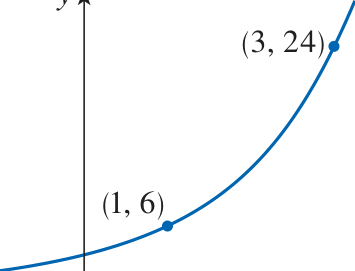
\includegraphics[width=\linewidth]{images/p0087_graph_2.png}
\end{minipage}\hfill
\begin{minipage}[t]{0.48\linewidth}
\textbf{20.}\\
\centering
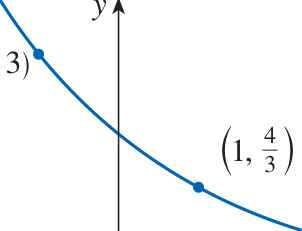
\includegraphics[width=\linewidth]{images/p0087_graph_3.png}
\end{minipage}

\vspace{0.6em}
\noindent\textbf{21.} Nếu $f(x) = 5^x$, hãy chứng minh rằng
\[
\frac{f(x + h) - f(x)}{h} = 5^x \left(\frac{5^h - 1}{h}\right)
\]

\vspace{0.4em}
\noindent\textbf{22.} Giả sử bạn được đề nghị một công việc kéo dài một tháng. Bạn sẽ ưu tiên phương thức thanh toán nào sau đây hơn?
\begin{enumerate}[label=\Roman*.,leftmargin=*,itemsep=1pt,topsep=2pt]
\item Một triệu đô la vào cuối tháng.
\item Một xu vào ngày đầu tiên của tháng, hai xu vào ngày thứ hai, bốn xu vào ngày thứ ba, và tổng quát là $2^{n-1}$ xu vào ngày thứ $n$.
\end{enumerate}

\vspace{0.4em}
\noindent\textbf{23.} Giả sử đồ thị của các hàm số $f(x) = x^2$ và $g(x) = 2^x$ được vẽ trên một hệ lưới tọa độ với đơn vị đo là $1\text{ inch}$. Hãy chứng minh rằng ở khoảng cách $2\text{ ft}$ về phía bên phải của gốc tọa độ, chiều cao của đồ thị hàm số $f$ là $48\text{ ft}$ nhưng chiều cao của đồ thị hàm số $g$ lên tới khoảng $265\text{ dặm (mi)}$.

\vspace{0.5em}
\noindent\raisebox{-1pt}{\tikz[scale=0.16]{\draw[line width=0.6pt, rounded corners=0.8pt] (0,0) rectangle (1.2,0.9); \draw[stewartcyan, line width=0.6pt] (0.2,0.2) to[out=10,in=250] (1.0,0.7); \draw[line width=0.6pt] (0.4,-0.2) -- (0.8,-0.2); \draw[line width=0.6pt] (0.6,0) -- (0.6,-0.2);}}\;\textbf{24.} So sánh các hàm số $f(x) = x^5$ và $g(x) = 5^x$ bằng cách vẽ đồ thị cả hai hàm số trong một số khung nhìn khác nhau. Tìm tất cả các giao điểm của các đồ thị chính xác đến một chữ số thập phân. Hàm số nào tăng nhanh hơn khi $x$ đủ lớn?

\vspace{0.5em}
\noindent\raisebox{-1pt}{\tikz[scale=0.16]{\draw[line width=0.6pt, rounded corners=0.8pt] (0,0) rectangle (1.2,0.9); \draw[stewartcyan, line width=0.6pt] (0.2,0.2) to[out=10,in=250] (1.0,0.7); \draw[line width=0.6pt] (0.4,-0.2) -- (0.8,-0.2); \draw[line width=0.6pt] (0.6,0) -- (0.6,-0.2);}}\;\textbf{25.} So sánh các hàm số $f(x) = x^{10}$ và $g(x) = e^x$ bằng cách vẽ đồ thị cả hai hàm số trong một số khung nhìn khác nhau. Khi nào thì đồ thị của $g$ cuối cùng sẽ vượt qua đồ thị của $f$?

\vspace{0.5em}
\noindent\raisebox{-1pt}{\tikz[scale=0.16]{\draw[line width=0.6pt, rounded corners=0.8pt] (0,0) rectangle (1.2,0.9); \draw[stewartcyan, line width=0.6pt] (0.2,0.2) to[out=10,in=250] (1.0,0.7); \draw[line width=0.6pt] (0.4,-0.2) -- (0.8,-0.2); \draw[line width=0.6pt] (0.6,0) -- (0.6,-0.2);}}\;\textbf{26.} Sử dụng đồ thị để ước lượng các giá trị của $x$ sao cho
\[
e^x > 1{,}000{,}000{,}000
\]

\end{multicols}